\documentclass[10pt,oneside,slovak,a4paper]{article}

\usepackage[slovak]{babel}
\usepackage[IL2]{fontenc}
\usepackage[utf8]{inputenc}
\usepackage{graphicx}
\usepackage{url}
\usepackage{xcolor}
\usepackage{hyperref}
\usepackage{listings}
\usepackage{refstyle}
\usepackage[font={small,it}]{caption}

\usepackage{fancyhdr}
\pagestyle{fancy}
\fancyhf{}

%hlavicka dokumentu
\rhead{ID: 110867 }
\lhead{Matej Pakán}
%paticka dokumentu
\fancyfoot[CE,CO]{Evolučné programovanie}
\fancyfoot[LE,RO]{\thepage}

\usepackage{listings}
\usepackage{color}

\definecolor{mygreen}{rgb}{0,0.6,0}
\definecolor{mygray}{rgb}{0.5,0.5,0.5}
\definecolor{mymauve}{rgb}{0.58,0,0.82}

\lstdefinestyle{customc}{
	firstnumber=1,
	stepnumber=1,
	numbers=left, 
  belowcaptionskip=1\baselineskip,
  breaklines=true,
  frame=L,
  basicstyle=\tiny,
  xleftmargin=\parindent,
  language=C,
  showstringspaces=false,
  basicstyle=\footnotesize\ttfamily,
  keywordstyle=\bfseries\color{green!40!black},
  commentstyle=\itshape\color{purple!40!black},
  identifierstyle=\color{blue},
  stringstyle=\color{orange},
}

\lstdefinestyle{customasm}{
  belowcaptionskip=1\baselineskip,
  frame=L,
  xleftmargin=\parindent,
  language=[x86masm]Assembler,
  basicstyle=\footnotesize\ttfamily,
  commentstyle=\itshape\color{purple!40!black},
}

\lstset{escapechar=@,style=customc}
%zdroj týchto nastavení': https://en.wikibooks.org/wiki/LaTeX/Source_Code_Listings     --upravené

\usepackage{cite}


\title{Evolučné programovanie\thanks{Riešenie 3. zadanie - Evolučné programovanie - hľadač pokladov – v predmete umelá inteligencia, ak. rok 2021/22, cvičiaci: 
Ing. Ivan Kapustík}}

\author{Matej Pakán\\[2pt]
	{\small ID: 110867}\\
	{\small Slovenská technická univerzita v Bratislave}\\
	{\small Fakulta informatiky a informačných technológií}\\
	{\small \texttt{xpakan@stuba.sk}}
	}

\date{\small 12. novembra 2021}



\begin{document}

\maketitle
\newpage
\tableofcontents{\protect\newpage}

\section{Zadanie}

Majme hľadača pokladov, ktorý sa pohybuje vo svete definovanom dvojrozmernou mriežkou (viď. obrázok) a zbiera poklady, ktoré nájde po ceste. Začína na políčku označenom písmenom S a môže sa pohybovať štyrmi rôznymi smermi: hore H, dole D, doprava P a doľava L. K dispozícii má konečný počet krokov. Jeho úlohou je nazbierať čo najviac pokladov. Za nájdenie pokladu sa považuje len pozícia, pri ktorej je hľadač aj poklad na tom istom políčku. Susedné políčka sa neberú do úvahy.

\begin{figure}[h]
\centerline{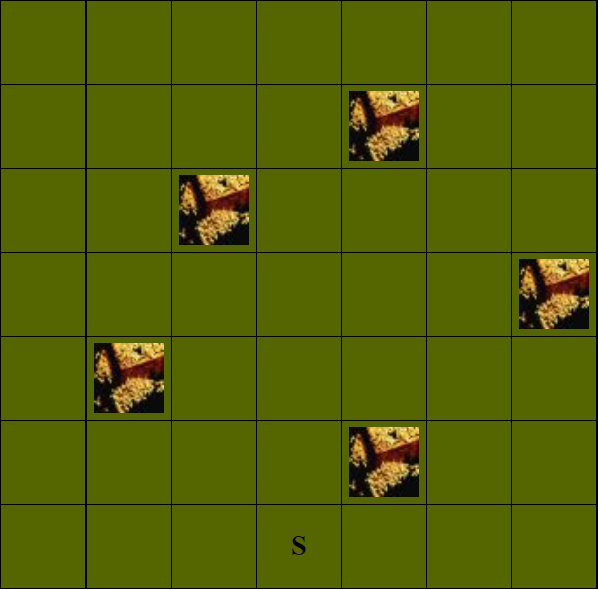
\includegraphics[scale=0.5]{./assets/zadanie.png}} 
\caption{Vzorové zadanie problému}
\end{figure}

Horeuvedenú úlohu riešte prostredníctvom evolučného programovania nad virtuálnym strojom.

Tento špecifický spôsob evolučného programovania využíva spoločnú pamäť pre údaje a inštrukcie. Pamäť je na začiatku vynulovaná a naplnená od prvej bunky inštrukciami. Za programom alebo od určeného miesta sú uložené inicializačné údaje (ak sú nejaké potrebné). Po inicializácii sa začne vykonávať program od prvej pamäťovej bunky. (Prvou je samozrejme bunka s adresou 000000.) Inštrukcie modifikujú pamäťové bunky, môžu realizovať vetvenie, programové skoky, čítať nejaké údaje zo vstupu a prípadne aj zapisovať na výstup. Program sa končí inštrukciou na zastavenie, po stanovenom počte krokov, pri chybnej inštrukcii, po úplnom alebo nesprávnom výstupe. Kvalita programu sa ohodnotí na základe vyprodukovaného výstupu alebo, keď program nezapisuje na výstup, podľa výsledného stavu určených pamäťových buniek.

\section{Úvodné nastavenia}

Hneď nazačiatok som si vytvoril funkciu na čítanie zadania zo súboru. Tieto údaje načítavam po celých riadkoch.
Na prvom riadku sa nachádza rozmer mriežky (7x7), na druhom je štartová pozícia hľadača (x,y).
Na zvyšných riadkoch až dokonca súbora načítavam súradnice pokladov (x,y).

Pre správnu funkčnosť som použil externé knižnice - random, time a math.

\section{Reprezentácia jedinca}

Každá \textbf{entita} (jedinec) obsahuje svoj \textbf{genóm} (zoznam génom), \textbf{fitness} (miera sily/úspešnosti jedinca) a \textbf{prints} (pohyb/výpis).

Object jedinca obsahuje aj funkciu vykonania pohybu po mriežke, k čomu sa dostaneme neskôr v dokumentácii.

\section{Generovanie prvej generácie}

Úvodnú generáciu generujem nasledovne:

Vytvorím si objekt \textbf{jedinca}. Tomuto jedincovi následne \textbf{vytváram 64 génov}. 

\begin{itemize}
\item{Tento gén, má následne na \textbf{prvých 2 bitoch zapísanú inštrukciu} tak, ako je napísané v zadaní (hodnoty od 00 po 11).}

\item{\textbf{Ďalších 6 bitov reprezentuje adresu genómu} (číslo od 0 do 63) v binárnej sústave.}

\item{Prvé 2 bity (inštrukcia) teda \textbf{rozhodujú} o tom, \textbf{aká inštrukcia sa vykonú nad ďalšími 6 bitmi} (adresa).}

\item{Takýto gén \textbf{pridávam do celkového genómu} (zoznam) jedinca.}

\item{Takto vytvoreného jedinca pridávam do 1. generácie.}
\end{itemize}

Následne spúštam funkciu virtuálneho stroja nad týmto jedincov a hneď potom daného jedinca ohodnotím a pridám mu tak fitness. - Viac o tejto časti je opísané v ďalšej sekcii.

Tento postup opakujem \textbf{100 krát} (počet jedincov v generácii).

Kód vytvorenia počiatočnej generácie:
\begin{lstlisting}
for count in range(N_IN_GENERATION):
    # Generating entity
    entity = Entity()
    entity.genome = []
    for i in range(64):
        # Generating random gene from 0 to 255
        gene_int = randint(0,255)
        gene_bin = bin(gene_int)[2:].zfill(8)

        # Adding genome to entity
        entity.genome.append(gene_bin)

    # Running VM on entity and getting fitness
    VM(entity)
    rateEntity(entity)
    
    # Adding entity into generation
    generation.append(entity)
\end{lstlisting}

\section{Virtuálny stroj}

Funkciu virtuálneho stroja potrebuje jedinca ako parameter.

Následne vykonáva akcie nad každým génom z genómu jedinca a tento gén modifikuje.

Ak sa na prvých 2 bitov genómu vyskytuje '00', vykoná inkrementácia adresy génu.
To znamená, že ak bolo v géne zapísané '001011', tak sa tento gén prepíše na '001100'.

Pri bitoch '01' - inštrukcia dekrementácie, funguje prepisovanie analogicky, akurát opačným smerom, teda odpočítavame.

Zaujímava je funkcia JUMP ('10'), v pri tejto funkcii daný gén ignorujeme skáčeme na gén, ktorý je zapísaný v adresovej časti JUMP gény.

Poslednou funkciou je výpis ('11'), ktorá vykonáva funkciu addDirection v objekte jedinca, teda mu pridáva ďalší krok, ktorý hľadač vykoná.
Smer pohybu jedinca je určený poslednými 2 bitmi génu. 

\begin{lstlisting}
    def addDirection(self,bits):
        direction = ""
        if(bits == '00'):
            direction = "H"
        elif(bits == '01'):
            direction = "D"
        elif(bits == '10'):
            direction = "P"
        elif(bits == '11'):
            direction = "L"
        self.prints.append(direction)
\end{lstlisting} 

Ak by sa mal tento virtuálny stroj zacykliť, máme na to podmienku, že ak stroj spraví viac ako 500 inštrukcií, virtuálny stroj skončí.

\section{Hodnotenie jedinca}

Na hodnotenie jedinca slúži funkcia rateEntity. Táto funkcia zoberie už existujúci zoznam výpisov/pohybov jedinca, ktorý predtým vygeneroval virtuálny stroj.

Následne prechádza každý z pohybov a zisťuje, či je tento pohyb možný (teda či náhodou hľadač nevybočil z mriežky).
Ak je táto podmienka splnená, vykoná sa pohyb v danom smere.
Po vykonaní tohto pohybu sledujeme, či sa daný jedinec nenachádza na mieste kde je poklad. Ak áno, tento poklad vyhlasujeme za nájdený aby ho hľadač nehľadal znovu a zvyšujeme mu jeho fitness o 1 bod. Pokiaľ hľadač nenašiel všetky poklady, resetujeme zoznam pokladov na pôvodné súradnice. Fitness ale už ostáva uložený.

\section{Evolučný algoritmus}

Pri generovaní každej ďalšej generácie využívam rovnaký postup.

\begin{itemize}
\item{Nakopírujem najlepších X jedincov do novej generácie}
\item{Krížim Y nádejných jedincov z predošlej generácie a pridávam ich do novej generácie}
\item{Vytvorím Z úplne nových, náhodných jedincov}
\item{Nad každým jedincom z generácie spúšťam virtuálny stroj}
\item{Hodnotím každého jedinca}
\item{Ak som nenašiel všetky poklady, opakujem tento postup}
\end{itemize}

\subsection{Elitarizmus}

Pri mojom programe využívam elitarizmus, nakoľko som s ním dosiahol optimálnejšie výsledky.
Elitarizmus spočíva iba v tom, že nakopíruje najlepších jedincov zo starej generácie do novej generácie bezo zmeny.

\subsection{Výber rodičov a turnajový systém}
Na začiatku kríženia jedincov si vyberiem rodičov. To je N najlepších jedincov z predošlej generácie.
Následne podľa konfigurácie v úvode programu dopĺnam počet jedincov krížením.

Výber rodičov prebieha turnajovým systémom, t.j.vyberiem 4 náhodným rodičov a vytvorím "pavúkový" eliminačný systém turnaja.
V každom súboji nádejných rodičov sa porovnáva fitness - ten lepší postupuje do ďalšieho kola turnaja.
Víťaz tohto turnaja sa následne stáva rodičom.

Tento turnaj opakujeme ešte druhý krát, kedže rodičia musia byť dvaja.

Následne týchto jedincov krížim.
Samotné kríženie spočíva v tom, že 64 krát doplním gén do genómu nového jedinca, tak že náhodne (50 na 50) doplním N-tý 1. rodiča alebo 2. rodiča.
Keď toto opakovanie skončí, mám vytvoreného nového jedinca s celým genónom. 

\subsection{Mutovanie jedincov}

Jedinec, ktorý bol vygenerovaný krížením má šancu mutovať (2\% alebo podľa konfigurácie pri každom géne).
Znamená to, že prechádzam genónom jedinca (64 génov) a pri každom genóme je šanca, že daní gén kompletne zmutuje - vytvorí sa nový gén.



\section{Vývoj fitness}

Hodnota fitness u mňa spočíva iba v počte nájdených truhlíc. Mám implementované vylepšovanie fitness aj na základe počtu krokov, ale výsledky mám pri použití počtu krokov horšie (z mne neznámeho dôvodu :( ).



\section{Testovanie}
Testovanie som realizoval na notebooku s procesorom i5-7300HQ pri frekvencii procesora 3.2 - 3.5GHz.


\medskip

Ako môžete vidieť na testovaní vzorového riešenia, výsledky neboli úplne konštantné.
Správne riešenia som našiel v 7 z 10 prípadoch, ak som generoval menej ako 10 000 generácií.
Najrýchlejšie mi algoritmus pracoval týchto nastaveniach:

\begin{itemize}
\item{Miera mutácie - 2\%}
\item{Elitarizmus - 20 jedincov}
\item{Výber rodičov pozostával zo 60 najlepších jedincov}
\item{V každej novej generácii som generoval 10 úplne nových jedincov}
\item{Turnajový systém bol využitý}
\end{itemize}

\medskip 

Pri výpise riešenia uvádzam pomocou akých krokov sa k riešeniu podarilo dostať pomocou vypísania jednotlivých krokov v zozname.

\subsection{Porovnanie parametrov a spôsobov selekcie}

Výsledky testovania môžete nájsť na konci tohto dokumentu.  

\section{Možné vylepšenia}
Určite by pomohlo, ak by sa mi podarilo lepšie implementovať zlepšovanie fitness na základe vykonaného počtu krokov jedinca. 

\end{document}



























